
\documentclass[oneside,a4paper]{article}
\usepackage{amssymb}
\usepackage{changepage}
\usepackage{apacite}
\usepackage{xcolor}
\usepackage{graphicx}
\usepackage{geometry}
\usepackage{subcaption}
\usepackage{amsmath}
\usepackage{float}
%\setcitestyle{aysep=}


\begin{document}

\title{Correcting Measurement Error in Categorical Data}
\date{}
\author{An-Chiao Liu}

\maketitle

\section{Introduction}
Measurement error is the difference between an observed value (indicator) and the true value. It is usually hard to detect measurement error when researchers only have a single source for a variable without any other information, while this does not mean the variable is error-free. In national statistical institutes (NSIs), several variables can be collected from different sources, for example, a register and a survey that both collect people’s gender. If the combined record is not consistent, then an error is detected. Therefore, measurement error can be easily detected by comparing combined datasets from multiple sources. 

Once errors are detected, how to correct them will become the problem. If auxiliary variables are available and clear relations between auxiliary variables and the true variable are known, then edit rules should be applied for correction \cite{Thebook}. However, the concrete rules of corrections are not always available and other methods have to be applied. For NSIs and many other researchers, the subsequent parameter estimate (for instance contingency table, percentage of categories, etc.) is the main thing that should be focused on, not the exact value in each observation. An approach that can produce unbiased parameter estimates will be preferred. Therefore, multiple imputation was introduced to measurement error problems.

Multiple imputation has proven to be a good approach to deal with measurement error \cite{cole, MILC, MO1}. The target variable’s values are imputed $m\geq 2$ times, and the parameter is estimated $m$ times as well. The benefit is that by checking the variation between the parameter estimates, the uncertainty of imputation can be inspected \cite{bible}. This method has been widely applied to missing value problems. Similar to measurement error, missingness is also a kind of error in datasets. Also, observed values with error can be seen as information that is partly missing. This makes the knowledge of correction for missing values also informative in measurement error issues \cite{MO1}.

Under the multiple imputation framework, many multiple imputation methods were developed with different assumptions and approaches. Example of such assumptions and approaches are, the assumed distribution of the true values, the estimation method of measurement error, and the random drawing mechanism from the posterior predictive distribution. This research focuses on two multiple imputation methods, namely multiple overimputation (MO) \cite{MO2, MO1} and multiple imputation latent class (MILC) \cite{MILC}, in a categorical target variable contaminated with measurement error. Since both methods provide a solution for measurement error by using multiple indicators and can be easily generalized to different data types, this comparison is informative.

Furthermore, applied scenarios for these two methods were not sufficient in the original research. In \citeA{MO2}, only a five-category variable with a certain amount of measurement error was examined under one of the measurement error estimation approaches. In \citeA{MILC}, only binary variables were applied and missing values were listwise deleted. The number of categories affects the quality of imputation, that is, more categories will result in a higher proportion of misclassification \cite{Kropko}. How exactly this affects the performance of MO and MILC is unknown. Therefore, in this research the effect of the number of categories was explored. Also, a complete examination of how the existence of missingness, different proportions of error, and different error mechanisms affect the performance of imputation are provided.

Different types of datasets are also provided in this research. Considering the MO and MILC proposed approaches and the possible available information in NSIs, three types of datasets were chosen: multiple indicators, indicators with an auxiliary variable, and indicators with a gold standard variable. An auxiliary variable is a variable related to the true value but does not share the same concept as the true value. For example, job tenure can be an auxiliary variable for true income estimation. Normally researchers do not know exactly how the auxiliary variable relates to the true variable, thus different amounts of relation were explored in this research. A gold standard variable is an indicator without measurement error. It is usually available for a small subsample of units that was produced by manual correction or was obtained from highly reliable sources. Both auxiliary variables and gold standard variables provide valuable information in multiple imputation models. Therefore, different data types are applied in this research. This provides a practical suggestion when researchers have different kinds of data type at hand. 
 
To summarize, the aim of this research is three-fold. Firstly, compare the performance of MO and MILC. Secondly, extend MO and MILC to different scenarios. Thirdly, apply different data types in MO and MILC. These aspects are examined by a simulation study. An application of the two methods using a dataset from Statistics Netherlands is also demonstrated. By this research, a guideline for future researchers to deal with measurement errors in categorical variables under different scenarios is provided. 

\section{Background}
This research aims to compare two methods, MO and MILC, in measurement error problems. Here I start from the common part of the two methods, then elaborate MO and MILC in more depth in the following sections.

\begin{figure}
    \centering
    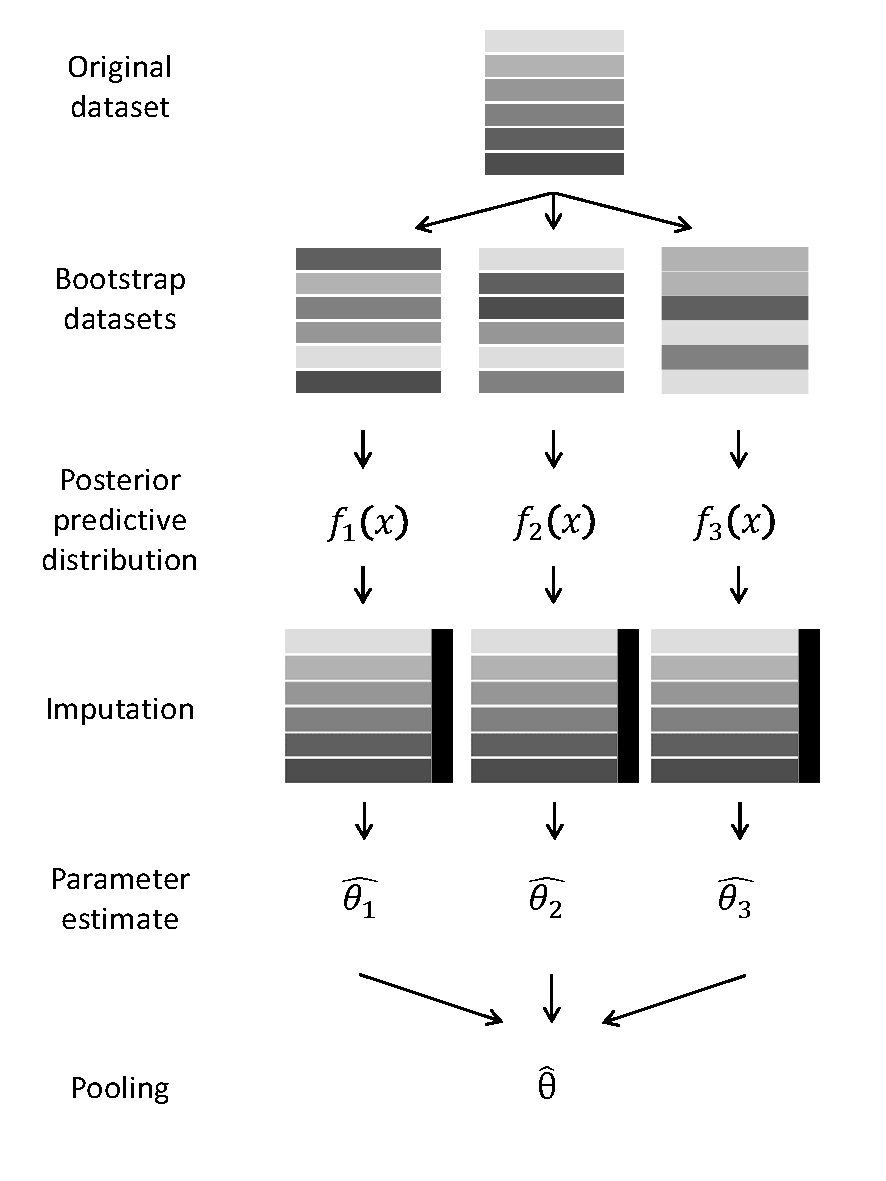
\includegraphics[width=0.4\textwidth]{MI.pdf}
    \caption{Multiple imputation process with $m=3$}
    \label{fig:MI}
\end{figure}
\subsubsection*{Multiple Imputation}
MO and MILC share the same multiple imputation process. Figure \ref{fig:MI} shows the process. Each of the methods assumes a distribution for the truth distribution, which is a linear model in MO and a latent class model in MILC.  Then, bootstrap the original dataset $m$ times to obtain $m$ datasets. In each dataset, combine information at the observation level (for example, observed indicators, auxiliary variables) with the assumed distribution to obtain $m$ posterior predictive distributions. Imputations are drawn from these $m$ posterior predictive distributions given the observation level information in the original dataset. Then, these $m$ imputations are combined with the original dataset for the computation of the subsequent parameter estimate ($\hat{\theta_i}$) which researchers are interested in (coefficient, mean, etc.). This parameter is estimated $m$ times and the estimates are pooled by Rubin’s rules \cite{Rubin1978}. That is, the overall point estimate ($\hat{\theta}$) is simply the mean of the $m$ estimates 
\begin{equation}
\hat{\theta}=\frac{1}{m}\sum_{i=1}^{m}\hat{\theta_i}.
\end{equation}
And the pooled variance of the estimate is a combination of variance within imputations and variances between imputations. That is,  
\begin{equation}
VAR_{total}=\overline{VAR}_{within}+VAR_{between}+\frac{VAR_{between}}{m}.
\end{equation}
The calculation of within variance is
\begin{equation}
\overline{VAR}_{within}=\frac{1}{m}\sum_{i=1}^{m}VAR_{within_i}.
\end{equation}
For categorical data, the variance for each category is calculated by
\begin{equation}
VAR_{within_i}=\frac{\hat{\theta_i} \times(1-\hat{\theta_i})}{N},\; \;
i \in\{1, 2, ...,m\},
\end{equation}
where N is the number of units in the dataset. The calculation of the variance between imputations is
\begin{equation}
VAR_{between}=\frac{1}{(m-1)}\sum_{i=1}^m(\hat{\theta_i}-\hat{\theta})^2.
\end{equation}

\subsubsection*{Assumptions of Data Type}
The following assumptions are taken into account for both MO and MILC when multiple indicators, an auxiliary variable, and a gold standard variable are available. Indicators are the observed values measuring the same latent trait, i.e. true value, we interested in. Both MO and MILC assume that the collection of indicators is independent. That is, for example, the reason causing errors to appear in a survey is not the same as the reason for errors in registration given the true values. Also, the quality of indicators is assumed to be unknown in this research, thus there is no weighting applied to indicators. This is not a necessary assumption when applying these two methods, but it is not in the scope of the discussion here.

Auxiliary variables are variables relevant to the true variable, which can facilitate the true value estimation and are assumed to be error-free. For example, owning a car or not can be used to estimate having a driving license or not. Both MO and MILC consider auxiliary variables in the posterior predictive distribution estimation. If auxiliary variables are available, it is crucial to combine auxiliary variables in the posterior predictive distribution. Since often the subsequent parameter estimates are relations of auxiliary variables and the indicators, these auxiliary variables should be included in the multiple imputation or else the parameter estimates will be biased \cite{meng}. \citeA{MO1} suggest that if other informative variables are available, even if they are not used in the parameter estimate, it is still worthwhile to include them in the imputation model to produce better estimates. Therefore, in the simulation study, the relation between how informative an auxiliary variable is and its contribution to imputation performance is shown. 

A gold standard variable is an error-free indicator. In NSIs, a small part of the observations in an indicator are manually checked for quality control. This research assumes that the probability of an observation having a gold standard variable is equal for all observations. Therefore, the relation between a gold standard variable and another indicator is assumed to be the same within observation. In the following subsections, the detail and the differences between MO and MILC will be elaborated.

\subsection{Multiple Overimputation}

Multiple overimputation (MO) corrects measurement error based on a linear model. MO treats every dataset as obtained from a multivariate normal distribution, even for categorical and ordinal variables. Two assumptions are made in MO: First, the presence of errors is irrelevant to the distribution of the true value and the distribution of the amount of error. This can be addressed as an expansion of missing at random (MAR) to ignorable measurement mechanism assignment (IMMA). Second, the distribution of the amount of error is assumed to be constant across observations. Under these assumptions, \citeA{MO1} proposed to separate indicators ($Y_{il}$) into the true value part ($X_{i}$) and the error part ($u_i$). That is,
\begin{equation}\label{mo}
Y_{il} = X_{i}+ u_{il}, \; \;
u_{il} | X_{i}  \sim \mathcal{N}(0,\sigma_{ul}^2).
\end{equation}
Here $i$ is the index of observations, and $l$ is the index of indicators. The indicator is assumed to be an unbiased estimate of the true value, and the variance of the error ($\sigma_{u}^2$) represents how much measurement error is included in the indicators and is assumed to be constant across observations. If the variance of the error is very large, any value can possibly be observed and the situation becomes similar to having a missing value. Note that when applying this approach to categorical variables, the order of the categories will affect the imputation result.  The closer a category is to the observed value, the higher the probability of this category to become the imputed value.

Three methods were proposed by \citeA{MO2,MO1} for the estimation of the variance of measurement error : 
\begin{enumerate}
\item By specifying a proportion of measurement error in the indicator. If the proportion of measurement error ($\rho$) is known from experience or the other literature, the error variance ($\sigma_{u}^2$) can be calculated by 
\begin{equation}
\hat{\sigma}_{u}^2 = \rho \times \hat{\sigma}_Y^2,
\end{equation}
where $\sigma_Y^2$ is the variance of the observed target indicator. Since it is rare to know the proportion of measurement error beforehand, this method was not applied in the simulation.
\item By using two indicators. Assuming that the variance of the true value is constant and the error in indicators is independent of the truth and independent of error in other indicators, the only common part within indicators is the truth’s variance. That is, when two observed indicators $Y_1$ and $Y_2$ are available, $Y_1$’s variance $\sigma_{Y1}^2 $ minus the covariance of  $Y_1$ and $Y_2$ will be the variance of measurement error in $Y_1$.
\begin{equation}
\hat{\sigma}_{u1}^2 = \hat{\sigma}_{Y1}^2 - cov(Y_{1},Y_{2}).
\end{equation}
\item By using a gold standard variable. This is similar to multiple indicators, the only difference is that the gold standard variable’s variance ($\sigma_g^2$)  is assumed to be an unbiased estimate of the true values’ variance. Therefore, the error variance is simply
\begin{equation}
\hat{\sigma}_{ul}^2 = \hat{\sigma}_{Yl}^2 - \hat{\sigma}_g^2.
\end{equation}
\end{enumerate}
In this research, the estimation of measurement error variance is generalised from two indicators to multiple indicators. When more than two indicators are available, a confirmatory factor analysis (CFA) can be applied for measurement error estimation \cite{SEM}. To elaborate on this, I start by explaining the assumptions in the second method mentioned above. Suppose two indicators $Y_1$ and $Y_2$ are on the same scale, from equation (\ref{mo}) we have:
\begin{equation}\label{ind}
\begin{split}
Y_{i1} = X_{i}+ u_{i1}, \; \;
&u_{i1} | X_{i}  \sim \mathcal{N}(0,\sigma_{u1}^2), \\
Y_{i2} = X_{i} + u_{i2}, \; \;
&u_{i2} | X_{i}  \sim \mathcal{N}(0, (p\sigma_{u1})^2).
\end{split}
\end{equation}
$p$ is an unknown parameter representing a different degree of measurement error in $Y_{i2}$ relative to $Y_{i1}$. It is assumed that $u_{i1}$ and $u_{i2}$ are independent and independent of $X_{i}$ as well (IMMA assumption). That is, 
\begin{equation}
\begin{split}
&cov(u_{1}, u_{2}) = 0 \\&cov(u_{1}, X) = 0\\&cov(u_{2}, X) = 0.
\end{split}
\end{equation}
Then the variances of $Y_{i1}$ and $Y_{i2}$ can be decomposed into 
\begin{equation}
\begin{split}
&\sigma_{Y1}^2 = \sigma_{X}^2 + \sigma_{u1}^2 \\
&\sigma_{Y2}^2 = \sigma_{X}^2 + (p\sigma_{u1})^2.
\end{split}
\end{equation}
Since the only common part within $\sigma_{Y1}^2$ and $\sigma_{Y2}^2$ is $\sigma_{X}^2$, the error variance of $Y_1$ therefore is
\begin{equation}
\sigma_{u1}^2 = \sigma_{Y1}^2 - cov(Y_{1},Y_{2})
\end{equation}
When $l$ $\geq3$ indicators are available, equation (\ref{ind}) becomes:
\begin{equation}
\textbf{Y}= \mathbf{ \Lambda }\textbf{X} + \textbf{u}, 
\end{equation}
\begin{equation*}
\textbf{Y} = 
\begin{bmatrix}
Y_1\\Y_2\\ \vdots \\Y_l
\end{bmatrix},\;
\mathbf{\Lambda}= 
\begin{bmatrix}
\lambda_1\\\lambda_2\\ \vdots \\\lambda_l
\end{bmatrix},\;
\textbf{X} = 
\begin{bmatrix}
x
\end{bmatrix},\;
\textbf{u} = 
\begin{bmatrix}
u_1\\u_2\\ \vdots \\u_l
\end{bmatrix},\;
\Phi= 
\begin{bmatrix}
\phi
\end{bmatrix},
\end{equation*}
where $\mathbf{\Lambda}$ is the coefficient matrix and $\Phi$ is the variance matrix of $\mathbf{X}$. Here only one latent variable $x$ is considered with its corresponding variance $\phi$. The variance-covariance matrix $\Sigma$ of $\textbf{Y}$ is
\begin{equation}
\Sigma =
\begin{bmatrix}
var(Y_1) &                           & \\
  cov(Y_1, Y_2) & var(Y_2)  & \\ 
              \vdots &    \vdots      \\       
     cov(Y_1, Y_l)&  \dots & &var(Y_l)  
\end{bmatrix},
\end{equation}
which can also be written as 
\begin{equation}
\Sigma =
\begin{bmatrix}
\lambda_1^2\phi + var(u_1)&                           & \\
 \lambda_1 \lambda_2 \phi & \lambda_2^2\phi + var(u_2)  & \\
              \vdots &   \vdots      \\             
  \lambda_1 \lambda_l \phi & \dots &\lambda_l^2\phi + var(u_l)
\end{bmatrix}.
\end{equation}
The unknown vectors $\Lambda$ and $\Phi$ can be estimated by a CFA model when more than three indicators are available \cite{SEM}. Also, when more than three indicators are available, it is not necessary to constrain indicators on the same scale as formula (\ref{ind}). The measurement error variance in each indicator then will be
\begin{equation}
var(u_l)=
\begin{bmatrix}
var(Y_1)-\lambda_1^2\phi\\var(Y_2)-\lambda_2^2\phi \\ \vdots\\var(Y_l)-\lambda_l^2\phi
\end{bmatrix}.
\end{equation}

The process of MO is as follows: First, calculate the measurement error variance by one of the methods above as a prior. Second, combining observation level information using Expectation-Maximization with a bootstrapping algorithm is used to find $m$ posterior predictive distributions. Once the posterior predictive distributions have converged, random draws from these $m$ posterior predictive distributions conditional on original data will become the imputed values. The parameter will be estimated $m$ times, and then the $m$ parameters are combined by Rubin's rules.

\subsection{Multiple Imputation Latent Class}
Multiple imputation latent class (MILC) assumes that the true value is a latent class variable with the same number of categories as the indicators, given that indicators are independent. The measurement error will not be estimated directly but reflects the latent class assignment probability. For example, if two out of three indicators’ values are equal, there is a high possibility that these two indicators contain the true value. Therefore, MILC might be problematic if the data contains too much measurement error.

To construct the posterior predictive distribution of the latent classes, information from the observation level is combined by Bayes’ rule. Then, calculate the conditional probability of the true value given the information we have. This can be formulated as follows, assuming $L$ indicators are available. Let $Y_l$ denote each indicator with $C$ classes, $\textbf{Y}$ denote a vector of $Y_l$ for each observation, and $\textbf{y}$ denote the corresponding observed values. $X$ denotes the true latent class with $x \in\{1,2,...,C\}$. Suppose the response pattern $P(\textbf{Y}=\textbf{y})$ is a weighted average of the X class specific probabilities $P(\textbf{Y}=\textbf{y}|X=x)$, that is,
\begin{equation}
P(\textbf{Y} = \textbf{y})=\sum_{x=1}^C P(X=x) P(\textbf{Y}=\textbf{y} | X=x).
\end{equation}
The assumption that the indicators are independent can be written as 
\begin{equation}
 P(\textbf{Y}=\textbf{y}| X=x) = \prod_{l=1}^L P(Y_l=y_l | X=x).
\end{equation}
Then, combining the two formulae above we have 
\begin{equation}
P(\textbf{Y}=\textbf{y}) = \sum_{x=1}^C P(X=x) \prod_{l=1}^L P(Y_l=y_l | X=x).
\end{equation}

The presence of missingness is also considered in this research. Existence of missing values in categorical data can be seen as an extra category “unknown”, that is, the number of classes in the indicators becomes $C+1$ while the number of classes in the truth variable remains $C$. 

When an auxiliary variable $Q$ is available, the above formula can be generalized into 
\begin{equation}
P(\textbf{Y} = \textbf{y} |Q=q) = \sum_{x=1}^C P(X=x | Q=q) \prod_{l=1}^L P(Y_l=y_l | X=x).
\end{equation}
The auxiliary variable is assumed to be independent of measurement error appearance, that is, there is no relation between $Y_l$ and $Q$ when considering $X$. 

In this research, the MILC model is also used in the scenario when a gold standard variable is available. Since a gold standard variable is an indicator without measurement error in part of the observations, it can be seen as one of the $Y_l$. Variable $\tau$ is introduced to indicate the observations with a gold standard, that is, $\tau_{ix} = 1$ represents that observation $i$ is known to belong to a true latent class $x$, and $\tau_{ix} = 0$ is the opposite. Considering $\tau$ we have
\begin{equation}
P(y_i | q_i,\tau_i) = \sum_{x=1}^C \tau_{ix} P(x | q_i) P(y_i | x).
\end{equation}

Expectation-Maximization algorithms and Newton-Raphson algorithms are used to estimate the parameters above. Then the posterior predictive distribution is obtained as
\begin{equation}
P(X=x|\textbf{Y} = \textbf{y}, Q = q) = \frac{P(X=x | Q = q) \prod_{l=1}^L P(Y_l = y_l | X = x)}{\sum_{x=1}^C P(X=x | Q = q)  \prod_{l=1}^L P(Y_l = y_l | X =x)}.
\end{equation}

To summarize, the process of MILC is as follows: First, bootstrap the original dataset $m$ times with the same sample size as the original dataset. Second, combine information with the latent class model and use Expectation-Maximization algorithms and Newton-Raphson algorithms to find the posterior predictive distributions in each dataset. Third, randomly draw a value from the $m$ posterior predictive distributions given observed data as imputations. Fourth, calculate parameter estimates for each of the $m$ imputed values. Finally, combine the parameter estimates by Rubin's rule.
 \section{Simulation}

\subsection{Data generation}
This simulation generated artificial data using R \cite{R}. The true values $X$ are generated from a random draw with equal probabilities within categories. The numbers of categories $C$ were 3, 6, 9 and the size of the generated dataset $N$ was 20,000. This large sample size was chosen because when 9 categories need to be estimated and missing values are present, $(9 +1 )^3*9 =9,000$ cells need to be estimated when we have 3 indicators. To have an acceptable model fit, preventing too many empty cells, a large sample size is needed.

The simulation considers the following four data types:
\begin{enumerate}
\item Three indicators.
\item Two indicators and a continuous auxiliary variable.
\item Two indicators and a categorical auxiliary variable.
\item Two indicators and a gold standard variable.
\end{enumerate}

To generate indicators, missingness and errors were imposed onto true values. Proportions of missingness were 0, 5\%, 10\%, and proportions of errors were 5\%, 15\%, 25\%. Random drawings from the true values under different proportions were selected to be missing or erroneous separately. Error values were filled in with an equal probability random draw from the possible categories other than the true value. For instance in the 3 categories scenario, if the truth is 1, then a random draw from 2 and 3 will be filled in as the error value. By this approach, missing completely at random (MCAR) and error completely at random were imposed. When the dataset includes auxiliary variables, missing at random (MAR) and ignorable measurement mechanism assignment (IMMA) were also imposed by members of missingness/error were related to the auxiliary variable.

Continuous and categorical auxiliary variables ($Q$) were generated by different correlations (0.2, 0.5, 0.8) with the true values. Different values of correlation reflect the information contained in the auxiliary variables. The auxiliary variables generation process was as follows. First, two continuous variables (A and B) were created under a multivariate normal distribution using the \texttt{MASS} package \cite{MASS} under $\sim \mathcal{N}(0,1)$ and the corresponding correlation with length $N$. Variable A was created to be a connection to the true value and B was the auxiliary variable to be created. Second, A was ordered and assigned to the same size as the true values in each category. For example, if the created truth has 30 observations in group 1, 40 observations in group 2, and 50 observations in group 3, then the smallest 30th observations in A are assigned to group 1, 31st to 70th are assigned to group 2 and so on. The corresponding variable B would be treated as the continuous auxiliary variable for each observation. For a categorical auxiliary variable, B was cut into the categories by order with equal size within groups. Corresponding to the former example it is 40 observations in each group. Note that by this method, true values and categorical auxiliary variables both contained order attributes.

A gold standard variable can be thought of as an indicator with a high proportion of missingness and without any error. In NSIs, the proportion of gold standard values is usually low due to the high cost of manual correction. Therefore, 5\% of the true values was randomly selected as the gold standard variable. 

\subsection{Multiple imputation}
MO was applied by means of the package \texttt{Amelia} \cite{Amelia}. One of the indicators was treated as the target imputed variable. The choice of the imputed indicator will slightly change the imputed value since the imputed indicator’s values were treated as prior means. Since the generation of each indicator did not differ from each other, the choice of which indicator to impute does not affect the conclusion. In the three indicators scenario, the measurement error variance was estimated by confirmatory factor analysis (CFA) by package \texttt{lavaan} \cite{lavaan}. The computed error variances were then plugged into \texttt{Amelia} as a prior variance to continue the further MO estimation. Furthermore, since MO treats categorical variables as continuous variables, the imputed values are also continuous. The imputed variables were rounded to the nearest category by using 0.5 as the cutoff point. 

Computation of MILC starts with bootstrapping the dataset into $m$ bootstrap samples, then estimates latent classes for each dataset. Latent class model were estimated by the \texttt{poLCA} package in R \cite{polca}, which also offers a function for drawing imputed values from the posterior predictive distributions.

The number of imputations (\textit{m}) was set to 10. \citeA{MO2} showed that the number of imputations does not affect the imputation performance in measurement error problems once it is over 10. \citeA{MILC} came to a similar conclusion as well.  

Proportions of each category were the parameters intended to be estimated. After imputation by MO or MILC, proportions of each category from imputed datasets were computed and pooled by Rubin’s rule. 

\subsection{Evaluation}
The number of the simulation was 10,000. The true proportion of each category is $1/C$ under different numbers of categories ($C$). Bias were computed by subtracting the pooled means from the true parameters. Mean squared errors (MSE) were also computed to evaluate the accuracy of the parameter estimation. 95\% confidence intervals were evaluated by looking at the proportion of the simulation containing the true value.

Model fit indicators were recorded in order to offer application suggestions. The relations between model fit indicators and the accuracy indicators (bias, MSE) were inspected, which can offer applied researchers an idea of how reliable their model is when applying these two methods. In MO, $R_{MO}^2$ was recorded as the model fit indicator. In MILC, entropy $R_{MILC}^2$ was computed by
\begin{equation}
Entropy\;R_{MILC}^2 = 1- \frac{EN(\alpha)}{N\,logC},
\end{equation}
where $N$ is the number of observations, $C$ is the number of categories. Entropy $EN(\alpha)$ is
\begin{equation}
EN(\alpha) = - \sum_{i=1}^N\sum_{x=1}^C \alpha_{ix}\, log \alpha_{ix},
\end{equation}
where $\alpha_{ix}$ is the probability that observation $i$ is a member of class $x$. Entropy $R_{MILC}^2$ is therefore between 0 and 1. When entropy $R_{MILC}^2$ close to 1, it means the observed probability is a perfect match with the latent class model.

 \section{Application}
MO and MILC were applied in the economic sectors’ energy usage dataset from Statistics Netherlands. Statistics Netherlands publishes statistics on economic sectors’ energy usage yearly, which includes the energy usage data (gas and electricity use of enterprises), and the SBI industry classification (in Dutch: Standaard Bedrijfsindeling). In the raw dataset, energy usage data is assumed to be error-free since it directly comes from network operators. Errors are present in the SBI codes because the datasets are linked and linkage error may be present, or because the original data sources were contaminated. This error can be detected by comparing SBI codes from different sources, but how to correct it is tricky and the result highly depends on the chosen model and assumptions. Actually, each company’s exact SBI code is not the main concern here. The focus is on producing reliable statistics to publish, therefore, multiple imputation may be suitable in this case since multiple imputation takes the uncertainty of the imputation into account.

The dataset contains records on about 1.6 million energy meters that belong to Dutch enterprises, including six indicators for SBI code, and two auxiliary variables. The parameter estimate was the mean energy usage in each economic sector, reported with 95\% confidence intervals.  

\bibliographystyle{apacite}
\bibliography{bibfile}

\end{document}



